% Template for ICME 2020 paper; to be used with:
%          spconf.sty  - ICASSP/ICIP/ICME LaTeX style file, and
%          IEEEbib.bst - IEEE bibliography style file.
% --------------------------------------------------------------------------
\documentclass{article}
\usepackage{spconf,amsmath,epsfig}
\usepackage{svg}

\let\OLDthebibliography\thebibliography
\renewcommand\thebibliography[1]{
  \OLDthebibliography{#1}
  \setlength{\parskip}{0pt}
  \setlength{\itemsep}{0pt plus 0.3ex}
}

\pagestyle{empty}


\begin{document}\sloppy

% Example definitions.
% --------------------
\def\x{{\mathbf x}}
\def\L{{\cal L}}


% Title.
% ------
\title{Chatroom Project}
%
% Single address.
% ---------------
\name{Gerard (Jed) Mijares, Andrew Perry}
%Address and e-mail should NOT be added in the submission paper. They should be present only in the camera ready paper. 
\address{}


\maketitle


%
\begin{abstract}
% The abstract should appear at the top of the left-hand column of text, about 0.5 inch (12 mm) below the title area and no more than 3.125 inches (80 mm) in length.  Leave a 0.5 inch (12 mm) space between the end of the abstract and the beginning of the main text.  The abstract should contain about 100 to 150 words, and should be identical to the abstract text submitted electronically along with the paper cover sheet.  All manuscripts must be in English, printed in black ink.



\end{abstract}
%
% \begin{keywords}
% One, two, three, four, five
% \end{keywords}
%
\section{Introduction}
\label{sec:intro}
A critical function of the internet has always been allowing people to communicate with each other remotely. This has been especially relevant this year, as it is more difficult to meet with people in person. Due to this, the group decided to create a chatroom application to explore this area firsthand. 

\subsection{Relevance to the Course}

(Should the textbook be cited somehow?)
The project most heavily builds on the content in Chapter 2 of the textbook. Specifically, the topics that were used are programming with sockets and sending messages or files back and forth. 

This project also relates to the material from Chapter 8. These topics are security and end-to-end encryption. 

Getting experience with these concepts helped to understand and reinforce the real-world applications where they are used. For example, seeing the effect that no encryption has on the security of the messages. Without any security, the messages could be easily intercepted and read with a packet sniffer such as Wireshark. Another example is splitting a large file into smaller chunks before sending. While this concept is learned early in this course, the act of actually programming and using this technique reinforces the concept.

\section{Literature Review}

\subsection{Comparison to Internet Relay Chat (IRC)}

Include the graphic from slide 4 of the slides! I need to learn how to do this. 

Internet Relay Chat (IRC), the first popularized open chat protocol (but not the first!) was invented in 1988 and still has users today. This is due to its...

Similar to our protocol, it operates on a client server scheme. Anybody who properly implements the protocol can connect to or create a server. 

Our protocol adds some features present in proprietary chat applications that are not available in "vanilla" IRC. (Though some users have created IRC extensions that add similar functions.)

Other open chat examples are XMPP and PSYC. 

\subsection{Comparison to Proprietary Applications}

Services such as Slack, Discord, and GroupMe are products offered that also offer chat applications. 

These applications are often robust and offer features that cater to a certain target market. For example, Slack is geared towards a professional work environment while Discord is designed for video game players to communicate. 

Unlike IRC and the chatroom application created for this project, these proprietary applications offer a standard client to use their service. It is not possible (or legal) to create a custom client to connect to these applications. However, some may offer Application Programming Interfaces (API) for people to create some sort of interface, such as bots. 

\section{Technical Approach Description}

% Will describe goals of project, as well as show and describe flow charts. Keeping some of the fluff below in case we want to use any of these. We could use them as examples. 

% Also kept the next long blurb so that I can copy/paste the formatting for quotes and such at some point. 

% An example of a bad paper:
% \begin{quote}
% \begin{center}
%     An analysis of the frobnicatable foo filter.
% \end{center}

%   In this paper we present a performance analysis of our
%   previous paper [1], and show it to be inferior to all
%   previously known methods. Why the previous paper was
%   accepted without this analysis is beyond me.

%   [1] Removed for blind review
% \end{quote}

% An example of an excellent paper:

% \begin{quote}
% \begin{center}
%      An analysis of the frobnicatable foo filter.
% \end{center}

%   In this paper we present a performance analysis of the
%   paper of Smith [1], and show it to be inferior to
%   all previously known methods.  Why the previous paper
%   was accepted without this analysis is beyond me.

%   [1] Smith, L and Jones, C. ``The frobnicatable foo
%   filter, a fundamental contribution to human knowledge''.
%   Nature 381(12), 1-213.
% \end{quote}

% If you are making a submission to another conference at the same time, which covers similar or overlapping material, you may need to refer to that submission in order to explain the differences, just as you would if you had previously published related work. In such cases, include the anonymized parallel submission~\cite{Authors12} as additional material and cite it as

% \begin{quote}
% 1. Authors. ``The frobnicatable foo filter'', ACM MM 2016 Submission ID 324, Supplied as additional material {\tt acmmm13.pdf}.
% \end{quote}

% Finally, you may feel you need to tell the reader that more details can be found elsewhere, and refer them to a technical report. For conference
% submissions, the paper must stand on its own, and not {\em require} the reviewer to go to a technical report for further details. Thus, you may say in
% the body of the paper ``further details may be found in~\cite{Authors12b}''.  Then submit the technical report as additional material. Again, you may not assume the reviewers will read this material.

% You can handle this paper like any other.  Don't write ``We show how to improve our previous work [Anonymous, 1968].  This time we tested the algorithm on a lunar lander [name of lander removed for blind review]''. That would be silly, and would immediately identify the authors. Instead write the following:
% \begin{quotation}
% \noindent
%   We describe a system for zero-g frobnication.  This
%   system is new because it handles the following cases:
%   A, B.  Previous systems [Zeus et al. 1968] didn't
%   handle case B properly.  Ours handles it by including
%   a foo term in the bar integral.

%   ...

%   The proposed system was integrated with the Apollo
%   lunar lander, and went all the way to the moon, don't
%   you know.  It displayed the following behaviours
%   which show how well we solved cases A and B: ...
% \end{quotation}

% \section{Design Points}

% A subsection for threading, encryption, and file sharing here. Show all of our pictures and find some way to incorporate our videos. 

\subsection{Threading}

At first, we approached the challenge with a simple procedural program on each end of the chatroom. We quickly found this was insufficient - users could indeed communicate with each other, but only if they took turns sending messages to each other. Otherwise the program would hang, not allowing the user to continue to send messages until they had received one.

To solve the problem, we redirected the chatroom program using a multi-threaded approach for both the client and server.

\subsection{Encryption}

Used a form of AES encryption, blah blah

\subsection{File Sharing}

Got these to add how I wanted them to, nice. 

\section{Experimental Results}

\section{Discussions on Results}

\section{Division of Labor}

Jed: Multi-threaded chat program, file transfer, and code flowcharts. 

Andrew: Encryption, encryption Wireshark experiment. 

\section{Conclusion}

To summarize, the project successfully completed all of our goals. We created a TCP chatroom program that is similar to IRC, while providing some extra features. 

Given more time, the next set of objectives would be as follows: 
\begin{itemize}
  \item Caching messages
  \item Private messages
  \item Improving robustness/error handling
  \item improved user interface, and
  \item Encryption/decryption of files. 
\end{itemize}

% \section{Major Headings}

% Major headings, for example, ``1. Introduction'', should appear in all capital letters, bold face if possible, centered in the column, with one blank line before, and one blank line after. Use a period (``.'') after the heading number, not a colon.

% \subsection{Subheadings}

% Subheadings should appear in lower case (initial word capitalized) in boldface. They should start at the left margin on a separate line.

% \subsubsection{Sub-subheadings}

% Sub-subheadings, as in this paragraph, are discouraged. However, if you must use them, they should appear in lower case (initial word capitalized) and start at the left margin on a separate line, with paragraph text beginning on the following line.  They should be in italics.

% \section{Page Numbering}

% Please do {\bf not} paginate your paper. Page numbers, session numbers, and conference identification will be inserted when the paper is included in the proceedings.

% Below is an example of how to insert images. Delete the ``\vspace'' line,
% uncomment the preceding line ``\centerline...'' and replace ``imageX.ps''
% with a suitable PostScript file name.
% -------------------------------------------------------------------------
%

\begin{figure}[h]
\caption{Example of a parametric plot ($\sin (x), \cos(x), x$)}
\centering
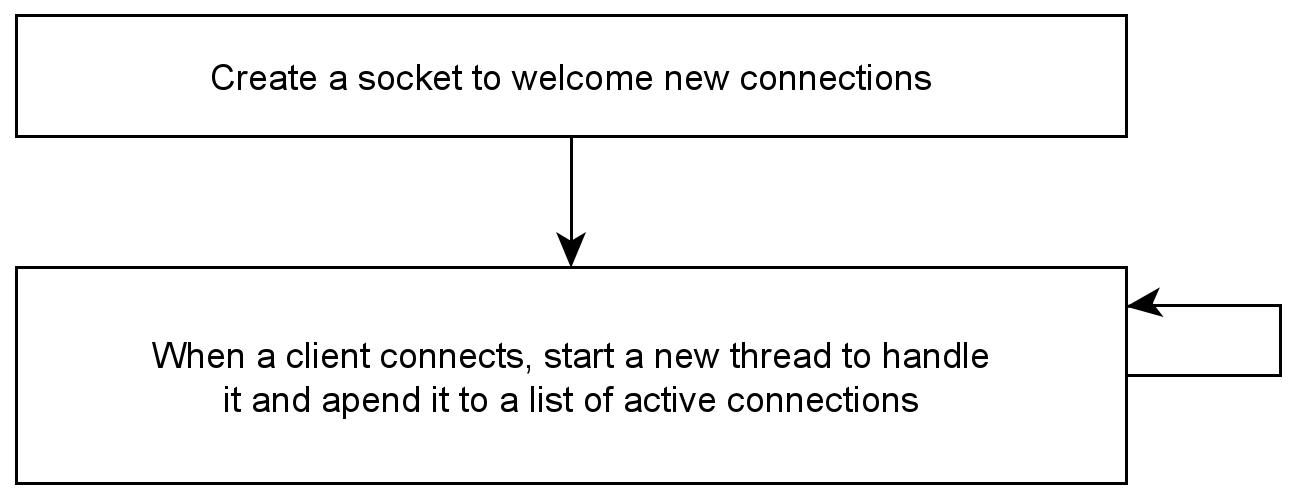
\includegraphics[width=0.5\textwidth]{media/serverFlowchart2.png}
\end{figure}

% \begin{figure}[t]
%     % \includesvg{media/serverFlowchart2}
% % \begin{minipage}[b]{1.0\linewidth}
% %   \centering
% % \centerline{\epsfig{figure=media/serverFlowchart2.svg,width=8.5cm}}
% %   \vspace{1.5cm}
% %   \centerline{(a) Result 1}\medskip
% % \end{minipage}
% % %
% % \begin{minipage}[b]{.48\linewidth}
% %   \centering
% % \centerline{\epsfig{figure=image3.ps,width=4.0cm}}
% %   \vspace{1.5cm}
% %   \centerline{(b) Results 2}\medskip
% % \end{minipage}
% % \hfill
% % \begin{minipage}[b]{0.48\linewidth}
% %   \centering
% % \centerline{\epsfig{figure=image4.ps,width=4.0cm}}
% %   \vspace{1.5cm}
% %   \centerline{(c) Result 3}\medskip
% % \end{minipage}
% % %
% \caption{Example of placing a figure with experimental results.}
% \label{fig:res}
% \end{figure}

% \section{Illustrations, Graphs, and Photographs}
% \label{sec:illust}

% Illustrations must appear within the designated margins. They may span the two columns. If possible, position illustrations at the top of columns, rather than in the middle or at the bottom. Caption and number every illustration. All halftone illustrations must be clear black and white prints.  Do not use any colors in illustrations.

% Since there are many ways, often incompatible, of including images (e.g., with experimental results) in a \LaTeX document. Figure~\ref{fig:res} shows you an example of how to do this.

% \section{Tables and Equations}

% Tables and important equations must be centered in the column. Table~\ref{tab:cap} shows an example of a table while the equation
% \begin{eqnarray}
% y &=& ax^2+bx+c \nonumber \\
% ~ &=& (x+p)(x+q)
% \end{eqnarray}
% shows an example of an equation layout.

% \begin{table}[t]
% \begin{center}
% \caption{Table caption} \label{tab:cap}
% \begin{tabular}{|c|c|c|}
%   \hline
%   % after \\: \hline or \cline{col1-col2} \cline{col3-col4} ...
%   Column One & Column Two & Column Three
%   \\
%   \hline
%   Cell 1 & Cell 2 & Cell 3 \\
%   Cell 4 & Cell 5 & Cell 6 \\
%   \hline
% \end{tabular}
% \end{center}
% \end{table}

% Large tables or long equations may span across both columns. Any table or equation that takes up more than one column width must be positioned either at the top or at the bottom of the page.

% \section{Footnotes}

% Use footnotes sparingly (or not at all!) and place them at the bottom of the column on the page on which they are referenced. Use Times 9-point type, single-spaced. To help your readers, avoid using footnotes altogether and include necessary peripheral observations in the text (within parentheses, if you prefer, as in this sentence).

% \section{Citations and References}

% List and number all bibliographical references at the end of the paper. The references can be numbered in alphabetic order or in order of appearance in the document. When referring to them in the text, type the corresponding reference number in square brackets as shown at the end of this sentence~\cite{Morgan2005}. All citations must be adhered to IEEE format and style. Examples such as~\cite{Morgan2005},~\cite{cooley65} and~\cite{haykin02} are given in Section 12.

% References should be produced using the bibtex program from suitable
% BiBTeX files (here: strings, refs, manuals). The IEEEbib.bst bibliography
% style file from IEEE produces unsorted bibliography list.
% -------------------------------------------------------------------------
\bibliographystyle{IEEEbib}
\bibliography{icme2020template}

\end{document}
